\section{宏包}

\begin{frame}[fragile]
\frametitle{加载宏包}
\begin{itemize}
  \item<+-> 「宏」包

    \begin{itemize}
      \item 提供扩展功能的组件
      \item 也就是别人造好的轮子
      \item 形式上为 |.sty| 扩展名的纯文本文件
    \end{itemize}

  \item<+-> 怎么用

    \begin{itemize}
      \item |\usepackage{ctex}|
      \item 小心载入顺序
    \end{itemize}

  \item<+-> 哪里找?

    \begin{itemize}
      \item The Comprehensive \TeX Archive Network \link{https://ctan.org/}
      \item GitHub
      \item<+-> 教程、博客、帖子(\alert{留意时效性})
    \end{itemize}
\end{itemize}
\end{frame}

\begin{frame}[fragile]
  \frametitle{宏包推荐(\textbf{先读文档}后使用)}
  % \vspace{-1em}
  \hspace{-3.5em}
  \begin{minipage}[t]{1.2\linewidth}%
    \begin{multicols}{3}
      \begin{itemize}
        \item 必备
  
          \begin{itemize}
            \item \pkg{amsmath公式}
            \item \pkg{graphicx插图}
            \item \pkg{hyperref超链接}
          \end{itemize}
  
        \item 样式
  
          \begin{itemize}
            \item \pkg{caption图注}
            \item \pkg{enumitem列表}
            \item \pkg{fancyhdr页眉页脚}
            \item \pkg{footmisc脚注}
            \item \pkg{geometry页面规格(纸张,边距)}
            \item \pkg{titlesec标题格式}
          \end{itemize}
  
        \item 数学
  
          \begin{itemize}
            \item \pkg{bm粗体数学符号}
            \item \pkg{mathtools公式增强}
            \item \pkg{physics物理符号增强}
            \item \pkg{unicode-math数学符号(unicode模式)}
          \end{itemize}
  
        \item 表格
  
          \begin{itemize}
            \item \pkg{array}
            \item \pkg{booktabs表格高级样式}
            \item \pkg{longtable跨页表格}
            \item \pkg{tabularx可变宽度表}
          \end{itemize}
  
        \item 插图、绘图
  
          \begin{itemize}
            \item \pkg{float}
            \item \pkg{pdfpages嵌入PDF}
            \item \pkg{standalone}
            \item \pkg{subfig子图片}
            \item \pkg{pgf}/\pkg{tikz流程图}
            \item \pkg{pgfplots通用数据作图}
          \end{itemize}
  
        \item 字体
  
          \begin{itemize}
            \item \pkg{newpx}
            \item \pkg{pifont}
            \item \pkg{fontspec引入/声明外部字体}
          \end{itemize}
  
        \item 各种功能
  
          \begin{itemize}
            \item \pkg{algorithm2e伪代码}
            \item \pkg{beamer幻灯片}
            \item \pkg{biblatex引文}
            \item \pkg{listings列表}
            \item \pkg{mhchem化学式}
            \item \pkg{microtype缩进控制}
            \item \pkg{minted代码高亮}
            \item \pkg{natbib印文}
            \item \pkg{siunitx度量衡}
            \item \pkg{xcolor定义颜色}
          \end{itemize}
  
        \item 多语言
  
          \begin{itemize}
            \item \pkg{babel}
            \item \pkg{polyglossia}
            \item \pkg{ctex}
            \item \pkg{xeCJK中日韩文字}
          \end{itemize}
      \end{itemize}
    \end{multicols}
  \end{minipage}
\end{frame}

\begin{frame}[fragile]{宏包示例: Tikz (画图)}
    \vspace{-2em}
        \begin{columns}
        \begin{column}{.6\textwidth}
        \lstset{language=[LaTeX]TeX}
        \begin{lstlisting}[basicstyle=\ttfamily\tiny]
\usetikzlibrary{positioning, arrows, shapes, shapes.multipart, backgrounds, calc, automata} %需先导入所需的tikz形状库
\tikzstyle{mcstate} = [state, fill=gray!20!white]
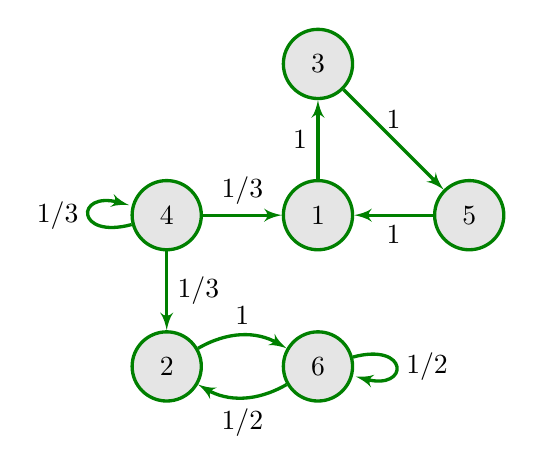
\begin{tikzpicture}[draw=Green, very thick, >=latex', auto]
    \node [mcstate]                 (s4) {4};
    \node [mcstate, right=of s4]    (s1) {1};
    \node [mcstate, below=of s4]    (s2) {2};
    \node [mcstate, right=of s2]    (s6) {6};
    \node [mcstate, right=of s1]    (s5) {5};
    \node [mcstate, above=of s1]    (s3) {3};
    
    \draw [->]
        (s4) edge [loop left] node {1/3} (s4)
        (s4) edge [above]     node {1/3} (s1)
        (s4) edge             node {1/3} (s2)
        (s1) edge             node {1} (s3)
        (s3) edge [above]     node {1} (s5)
        (s5) edge             node {1} (s1)
        (s2) edge [bend left] node {1} (s6)
        (s6) edge [bend left] node {1/2} (s2)
        (s6) edge [loop right] node {1/2} (s6);
\end{tikzpicture}                
        \end{lstlisting}
        \end{column}
        \begin{column}{.4\textwidth}
            \begin{figure}[H]
                \centering
                \tikzstyle{mcstate} = [state, fill=gray!20!white]
                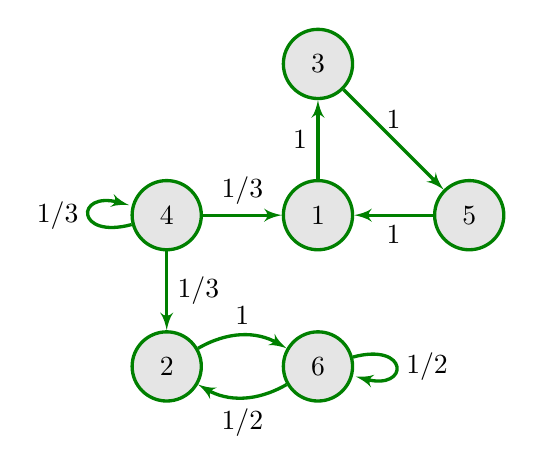
\begin{tikzpicture}[draw=Green, very thick, >=latex', auto]
                    \node [mcstate]                 (s4) {4};
                    \node [mcstate, right=of s4]    (s1) {1};
                    \node [mcstate, below=of s4]    (s2) {2};
                    \node [mcstate, right=of s2]    (s6) {6};
                    \node [mcstate, right=of s1]    (s5) {5};
                    \node [mcstate, above=of s1]    (s3) {3};
                    
                    \draw [->]
                        (s4) edge [loop left] node {1/3} (s4)
                        (s4) edge [above]     node {1/3} (s1)
                        (s4) edge             node {1/3} (s2)
                        (s1) edge             node {1} (s3)
                        (s3) edge [above]     node {1} (s5)
                        (s5) edge             node {1} (s1)
                        (s2) edge [bend left] node {1} (s6)
                        (s6) edge [bend left] node {1/2} (s2)
                        (s6) edge [loop right] node {1/2} (s6)
                    ;
                \end{tikzpicture}                
                \caption{Markov Chain} 
                \end{figure}
                    
        
        \end{column}
        \end{columns}
    Ref: \url{https://github.com/paulzfm/TikZ-Tunight} and TUNA 的有关讲座\link{https://tuna.moe/event/2020/tikz/}
    
\end{frame}

\begin{frame}[fragile]{宏包示例: \pkg{algorithm2e} (伪代码)}
    \begin{columns}
    \begin{column}{.6\textwidth}
        \lstset{language=[LaTeX]TeX}
    \begin{lstlisting}[basicstyle=\ttfamily\footnotesize]
\begin{algorithm}[H]
    \SetAlgoLined
    \LinesNumbered
    \SetKwInOut{Input}{input}
    \SetKwInOut{Output}{output}
    \Input{x: float, y: float}
    \Output{r: float}
    \While{True}{
        r = x + y\;
        \eIf{r >= 30}{
        ``O valor de $r$ é maior ou iqual a 10.''\;
        break\;
        }{
        ``O valor de $r$ = '', r\;
        }
        } 
        \caption{Algorithm Example}
\end{algorithm}
    \end{lstlisting}
    \end{column}
    \begin{column}{.4\textwidth}
        \begin{algorithm}[H]
            \SetAlgoLined
            \LinesNumbered
            \SetKwInOut{Input}{input}
            \SetKwInOut{Output}{output}
            \Input{x: float, y: float}
            \Output{r: float}
            \While{True}{
              r = x + y\;
              \eIf{r >= 30}{
               ``O valor de $r$ é maior ou iqual a 10.''\;
               break\;
               }{
               ``O valor de $r$ = '', r\;
              }
             } 
             \caption{Algorithm Example}
        \end{algorithm}
    \end{column}
    \end{columns}
\end{frame}